\documentclass[xcolor=table, handout]{beamer}

\usepackage{shyne}

% Theme settings
\setbeamertemplate{navigation symbols}{}

\usetheme{Madrid}
\usefonttheme{structurebold}
\usefonttheme[onlymath]{serif}

\AtBeginSection[]
{ 	\begin{frame}{}

	{
	\usebeamerfont{frametitle}
	\begin{beamercolorbox}
		[wd={\textwidth}, center, sep=.2in, rounded=true, shadow=true]
		{frametitle}
	Chapter \thesection\\  \secname 
	\end{beamercolorbox}
	}
	
	\end{frame} 
}

\AtBeginSubsection[]
{ 	\begin{frame}{}

	{
	\usebeamerfont{frametitle}
	\begin{beamercolorbox}
		[wd={\textwidth}, center, sep=.2in, rounded=true, shadow=true]
		{frametitle}
	Section \thesection .\thesubsection\\  \subsecname 
	\end{beamercolorbox}
	}
	
	\end{frame} 
}



\title[Chapter 6]{Stat 201: Statistics I\\ Chapter 6 }
\author[M. Shyne]{}
\institute[Metro State]{
\includegraphics[width=1.75in]{../images/metro_logo}}
\date[6/9/2019]{
\\ \bigskip \bigskip 
\includegraphics[width=.4in]{../images/cc_big}}


\begin{document}
\frame{\titlepage}

% Chapter 6
\setcounter{section}{5}
\section{Normal Probability Distributions}

% Section 6.1
\subsection{The Standard Normal Distribution}

\begin{frame}{Continuous probability distributions}
\begin{block}{}
{\large A \bt{continuous probability distribution} is a description of the probabilities of all possible values of a continuous random variable.}
\begin{itemize}
\pause\item Unlike discrete probability distributions, cannot be displayed in a table. There are infinite possible values.
\pause\item Distributions are precisely defined by a probability density function (PDF) or a cumulative density function (CDF).
\pause\item Probabilities of single values are technically always zero, $P(X=x)=0$.
\pause\item Only probabilities of ranges of values have meaning.
\end{itemize}
\end{block}
\end{frame}

\begin{frame}{Density curves}
\begin{block}{}
{\large A continuous probability distribution is visualized by a \bt{density curve}, a graph of the probability density function.}
\begin{itemize}
\item The total area under the graph is always 1.
\item Probabilities are defined as the area under the curve for the range of values of the random variable.
\end{itemize}
\end{block}
\medskip
{\centering
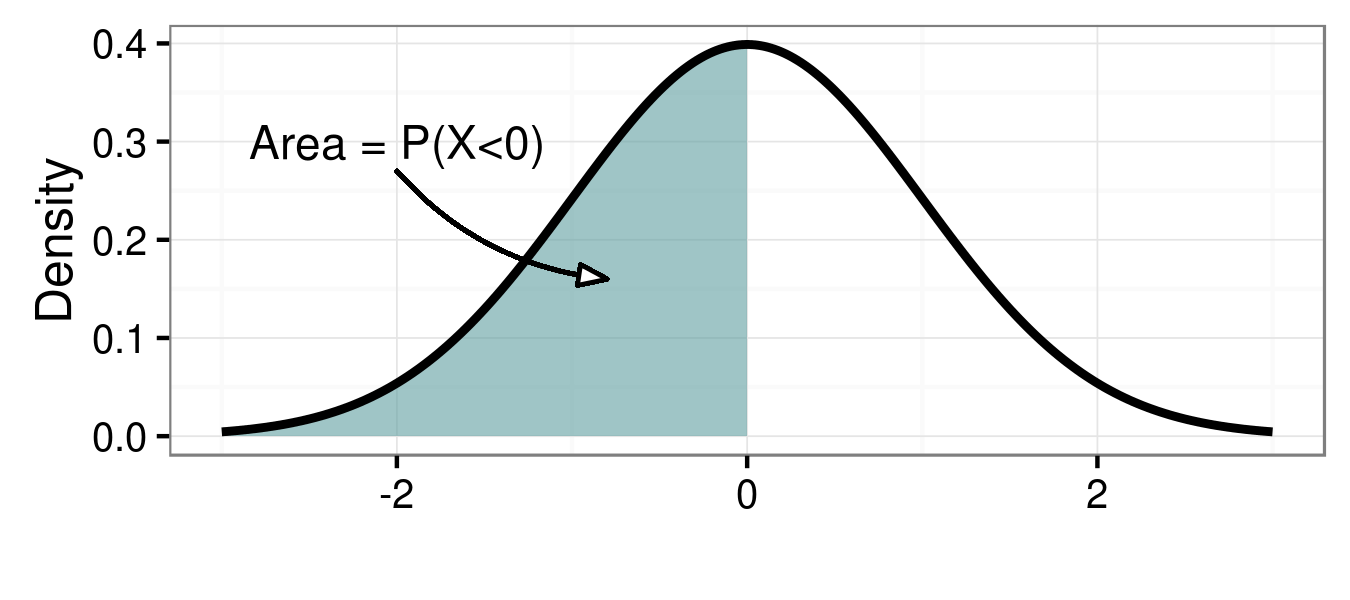
\includegraphics[width=4.5in]{../images/ch6_density_curve}
\par}
\end{frame}

\begin{frame}{Uniform probability distribution}
\begin{block}{}
{\large A random variable has an \bt{uniform distribution} if all possible values are equally likely.}
\begin{itemize}
\pause\item $X \sim U(a,b)$, $a$ is the minimum and $b$ is the maximum
\pause\item PDF: $f(x) = c$, where $c$ is a constant ($c = 1/(b-a)$)
\pause\item $P(u < x < v)$ is the area of the rectangle $(v-u) \times c$, or\\
\smallskip
{\centering $\ds P(u < x < v) = \frac {v-u}{b-a}$ \par} 
\end{itemize}
\end{block}
\smallskip
{\centering
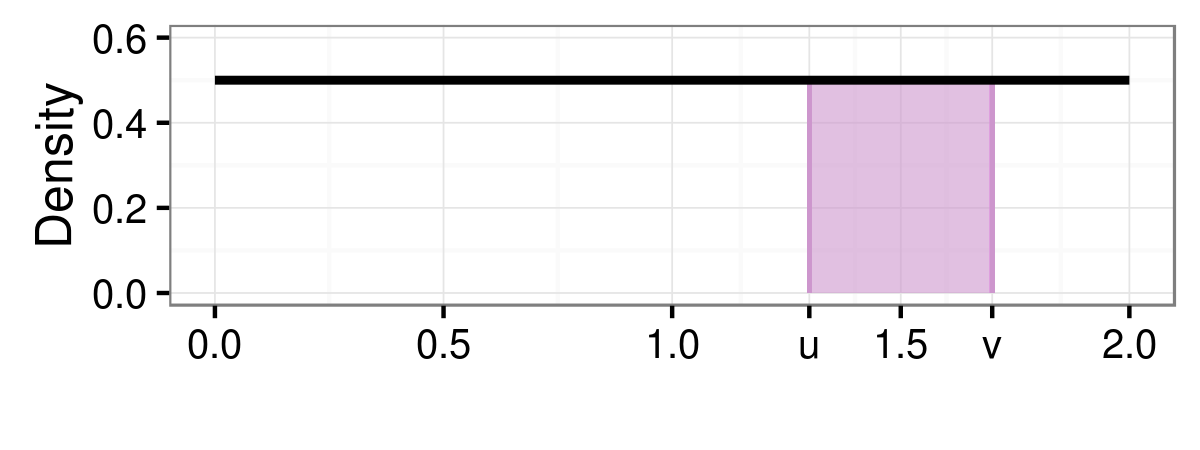
\includegraphics[width=4.5in]{../images/ch6_uniform}
\par}

\end{frame}

\begin{frame}{Uniform probability distribution, example}
\begin{exampleblock}{Example}
Bernice is waiting at the bus stop in a torrential downpour. She knows the bus will arrive any time between 0 and 30 minutes with equal likelihood. What is the probability she will have to wait between 5 and 15 minutes?\\
\smallskip
{\centering
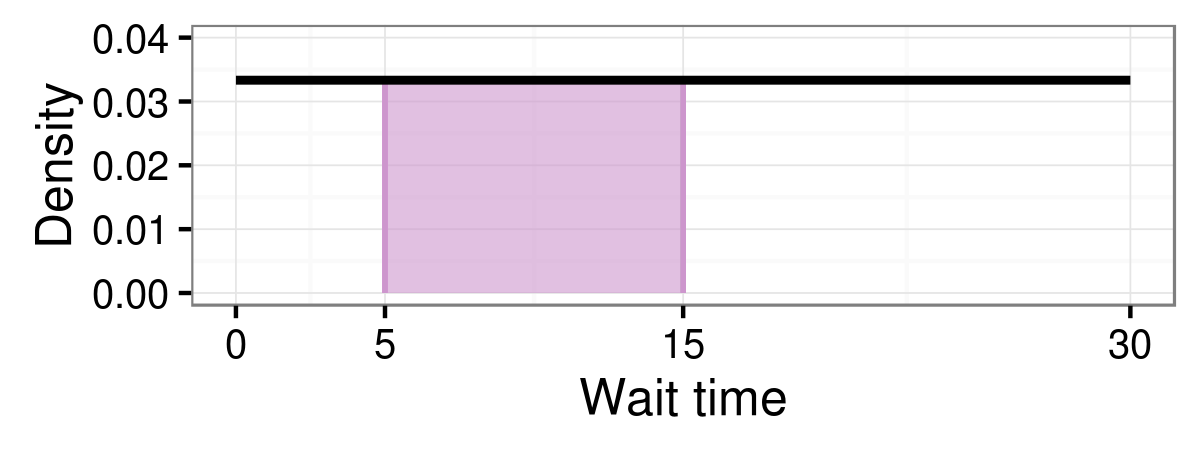
\includegraphics[width=4in]{../images/ch6_bus}
\par}
\begin{itemize}
\pause\item $X \sim U(0,30)$
\pause\item $\ds P(5 < X < 15) = \frac{15-5}{30-0} = \frac 1 3 = 0.33$
\end{itemize}
\end{exampleblock}
\end{frame}

\begin{frame}{Normal distributions}
\begin{block}{}
Recall, normal distributions were defined as having a particular shape.
\begin{itemize}
\item Start with low values, rise to a maximum value, and end with low values.
\item Distribution is symmetric (mirror image) around maximum.
\item ``Bell curve"
\end{itemize}
\end{block}

\pause
\begin{block}{}
Formally, random variable $X$ has a normal distribution with mean $\mu$ and standard deviation $\sigma$...
\begin{itemize}
\item $X \sim N(\mu, \sigma)$
\pause\item PDF: $\ds f(x\mid\mu, \sigma) = \frac 1 {\sqrt{2\pi} \sigma} e^{-\frac{(x-\mu)^2}{2\sigma}}$
\pause\item $\ds P(a <x < b \mid \mu, \sigma) = \frac 1 {\sqrt{2\pi} \sigma} \int_a^b e^{-\frac{(x-\mu)^2}{2\sigma}} \dd x$
\end{itemize}
\end{block}
\end{frame}

\begin{frame}{Symmetry of normal distribution}
\begin{block}{}
Normal distributions are perfectly symmetrical, mathematically speaking. That means, the probability a value is greater than some number is equal to the probability of being below the negative of that number.
\begin{itemize}
\item $P(X>c) = P(X < -c)$
\end{itemize}
\end{block}
\smallskip
{\centering
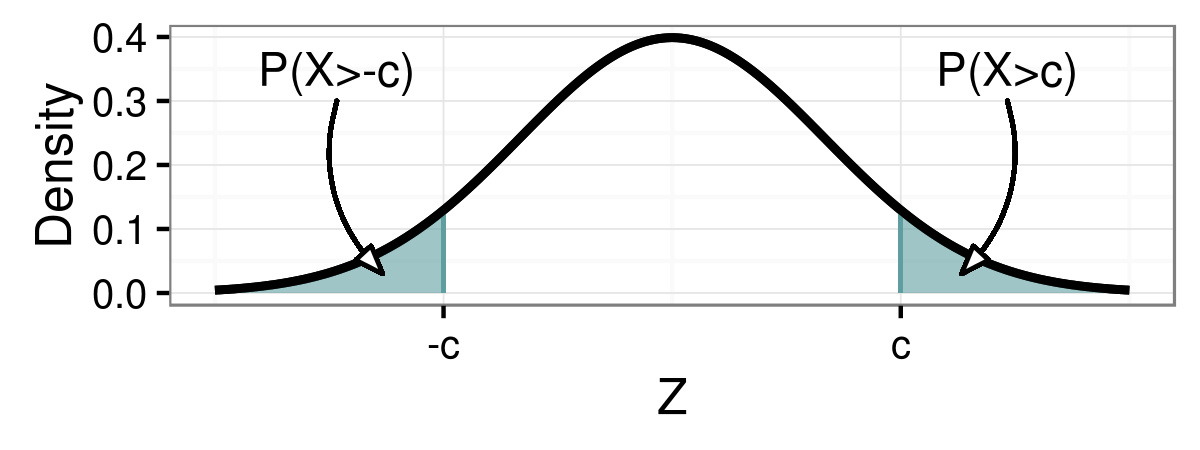
\includegraphics[width=4.5in]{../images/ch6_sym}
\par}

\end{frame}

\begin{frame}{Distribution of normal distributions}

\bigskip
{\centering
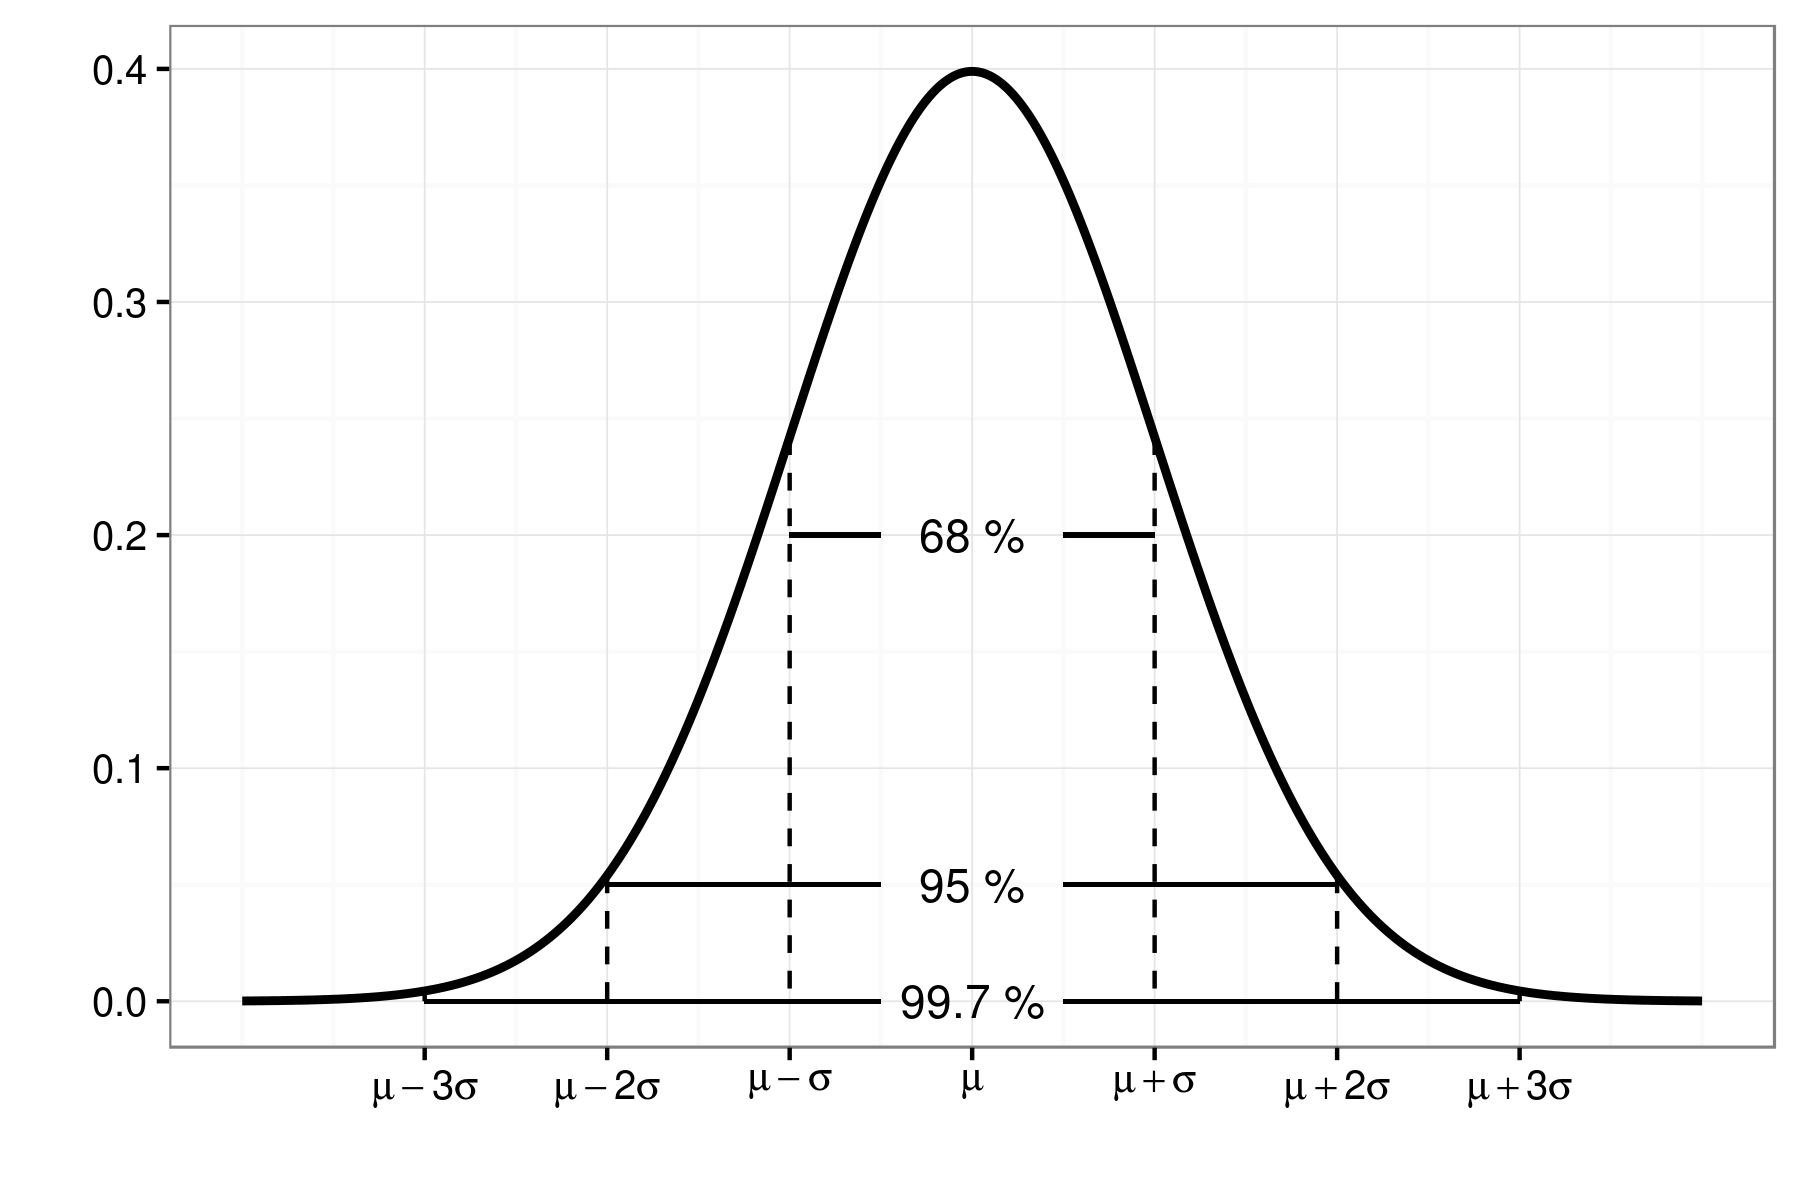
\includegraphics[width=4.5in]{../images/ch6_normal}
\par}

\end{frame}

\begin{frame}{Standard normal distribution}
\begin{block}{}
{\large A \bt{standard normal distribution} is a normal distribution with a mean $\mu=0$ and a standard deviation $\sigma =1$.  }
\begin{itemize}
\pause\item Also known as the $Z$ distribution.
\pause\item $Z \sim N(0,1)$
\pause\item Values of the standard normal are known as $z$-scores.
\pause\item A $z$-score of 1 ($z=1$) is one standard deviation above the mean, $z=-2$ is two standard deviations below the mean, etc.
\end{itemize}
\end{block}
\end{frame}

\begin{frame}{Z distribution}

\bigskip
{\centering
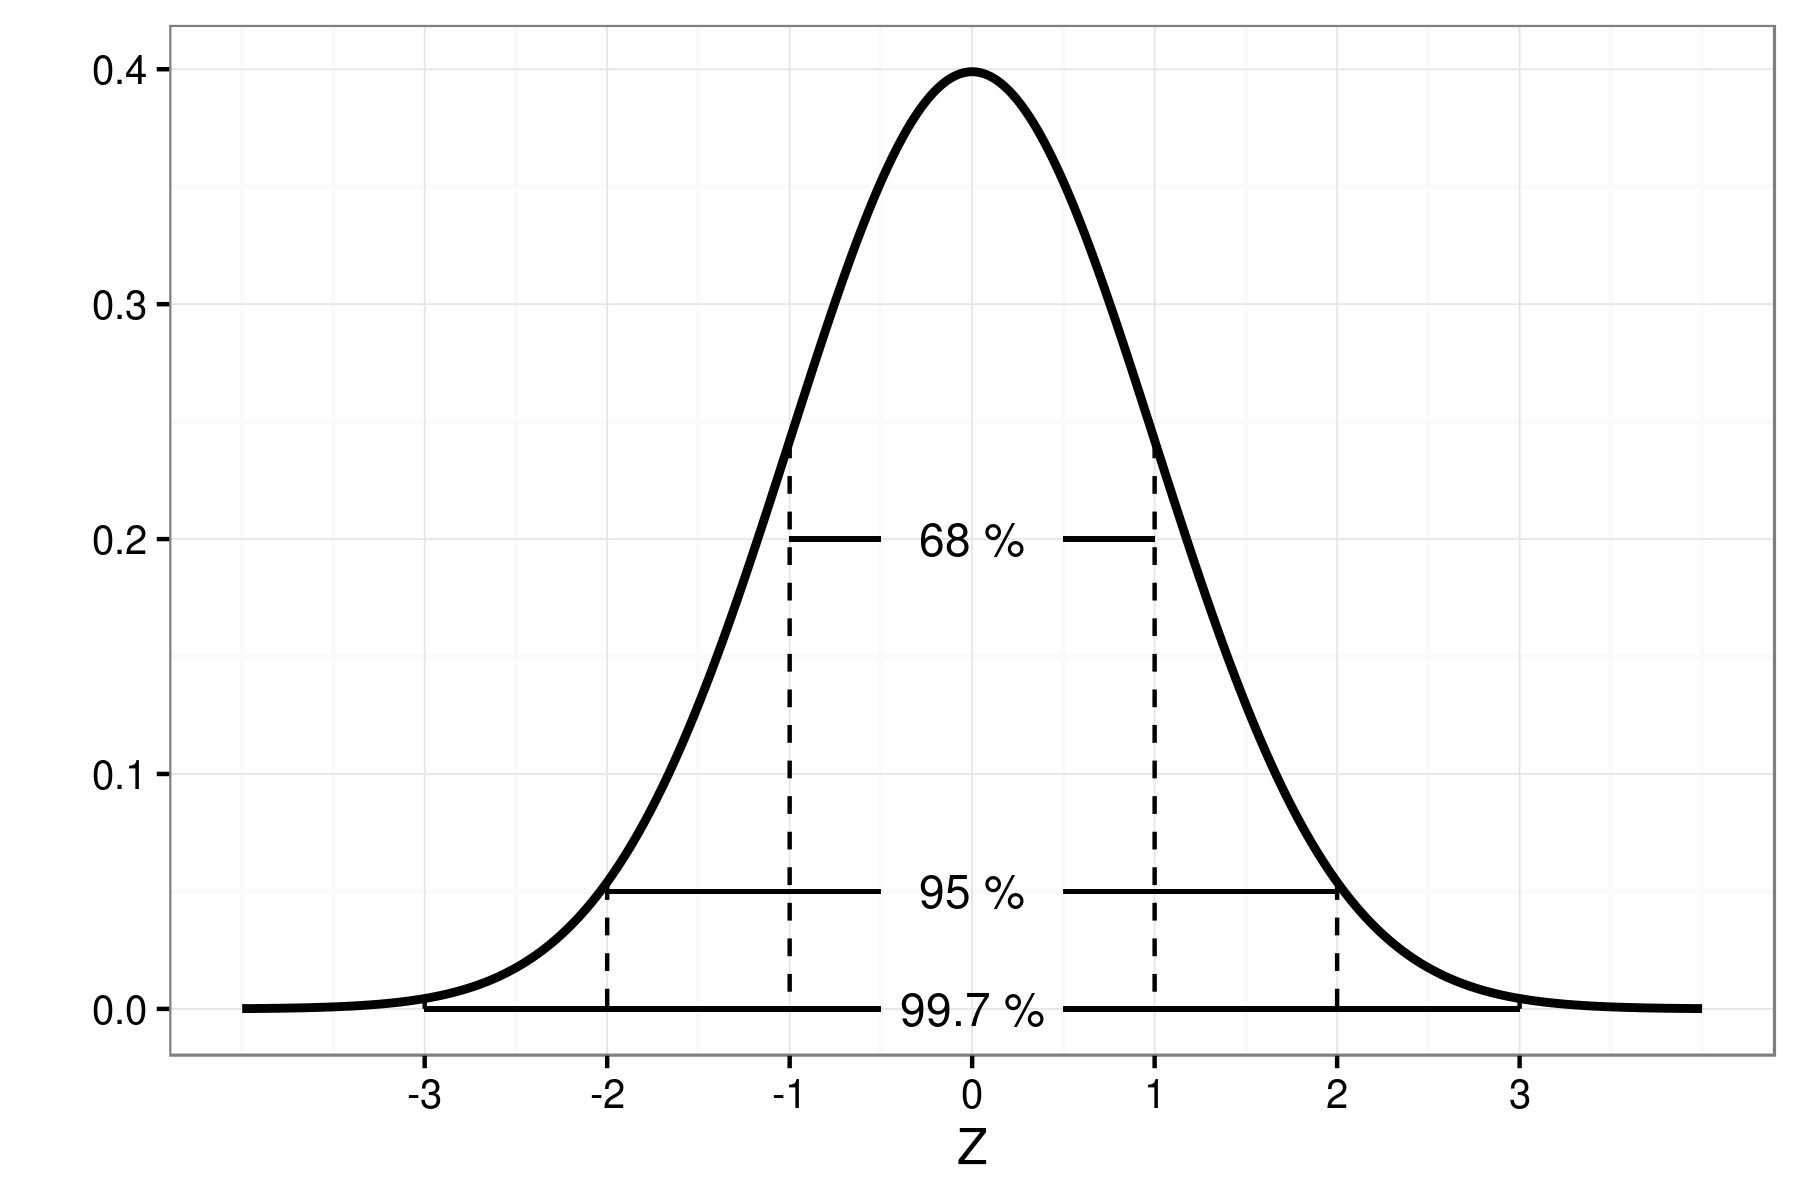
\includegraphics[width=4.5in]{../images/ch6_zdist}
\par}
\end{frame}

\begin{frame}{Probabilities of standard normal variables}
\begin{block}{}
Before technological resources, such as computers or statistical calculators, were widely available, tables (like Table A-2 in the book) were used to determine probabilities of events of normal random variables.
\begin{itemize}
\pause\item The table gives the probability for values less than a specified $z$-score, $P(Z < z)$
\pause\item To find probabilities for values greater than a specified $z$-score, subtract table probability from one, $P(Z > z) = 1-P(Z<z)$
\pause\item To find probabilities of ranges of values, subtract lower probability from higher, $P(z_1 < Z < z_2) = P(Z < z_2) - P(Z < z_1)$
\end{itemize}
\medskip
\pause However, using technology is usually quicker and more accurate.
\end{block}
\end{frame}


\begin{frame}{Probabilities, example}
\begin{exampleblock}{Example}
Using the standard normal distribution, find the probability a value is less than 0.75 standard deviations above the mean, $P(Z < 0.75)$\\
\smallskip
{\centering
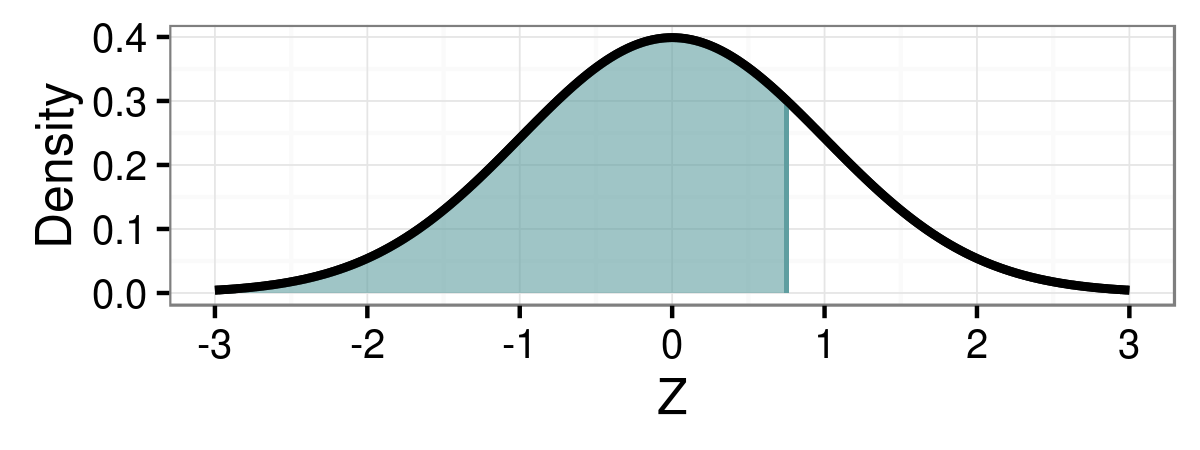
\includegraphics[width=4in]{../images/ch6_ex01}
\par}
\begin{itemize}
\pause\item $P(Z < .75) = \bv{0.773}$
\end{itemize}
\end{exampleblock}
\end{frame}

\begin{frame}{Probabilities, example}
\begin{exampleblock}{Example}
Using the standard normal distribution, find the probability a value is greater than 1.3 standard deviations below the mean, $P(Z > -1.3)$\\
\smallskip
{\centering
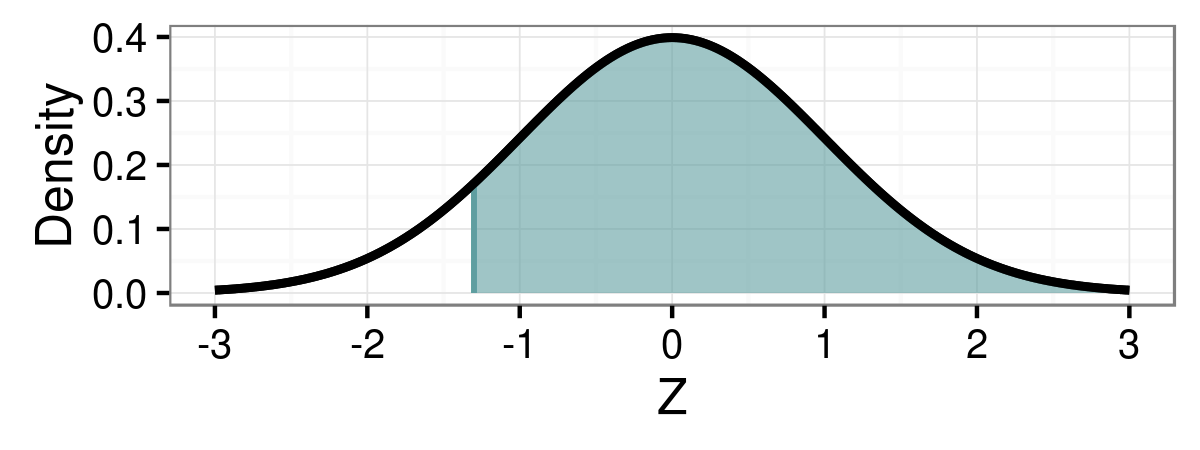
\includegraphics[width=4in]{../images/ch6_ex02}
\par}
\begin{itemize}
\pause\item $P(Z > -1.3) = \bv{0.903}$
\end{itemize}
\end{exampleblock}
\end{frame}

\begin{frame}{Probabilities, example}
\begin{exampleblock}{Example}
Using the standard normal distribution, find the probability a value is between -0.2 and 1.1 standard deviations, $P(-0.2 < Z < 1.1)$\\
\smallskip
{\centering
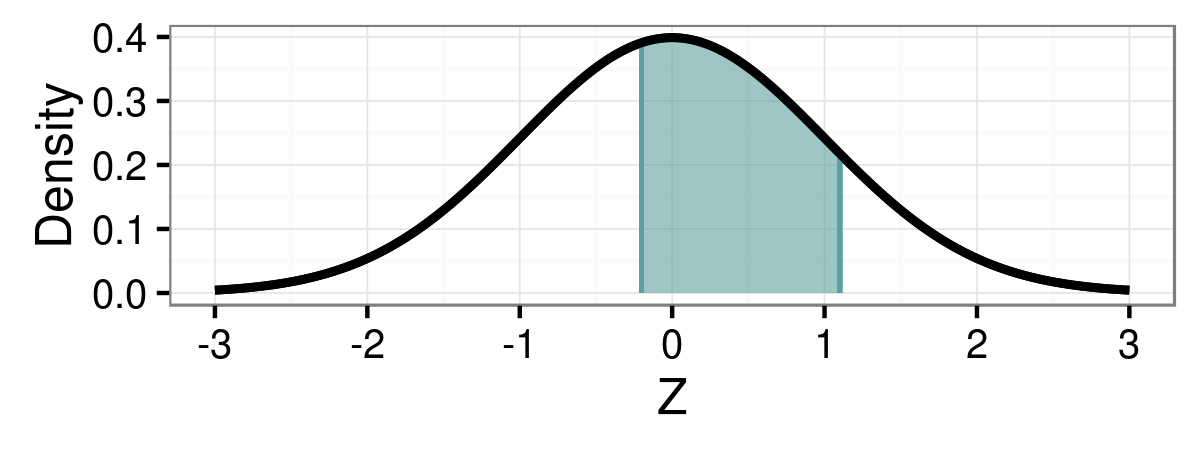
\includegraphics[width=4in]{../images/ch6_ex03}
\par}
\begin{itemize}
\pause\item $P(-0.2 < Z < 1.1) = \bv{0.444}$
\end{itemize}
\end{exampleblock}
\end{frame}

\begin{frame}{Finding percentiles}
\begin{block}{}
Often it is desirable to find a $z$-score that is greater than a specified probability, in other words, a percentile. This can be accomplished with the table by locating the desired probability and finding the corresponding $z$-score.\\
\medskip
Again, technology provides an easier and more accurate method.
\end{block}
\end{frame}

\begin{frame}{Finding percentiles, example}
\begin{exampleblock}{Example}
What is the z-score greater than 35\% of values? What is $P_{35}$? For what $z$-score is there a 0.35 probability of being less than $P(Z < z) = 0.35$?\\
\smallskip
{\centering
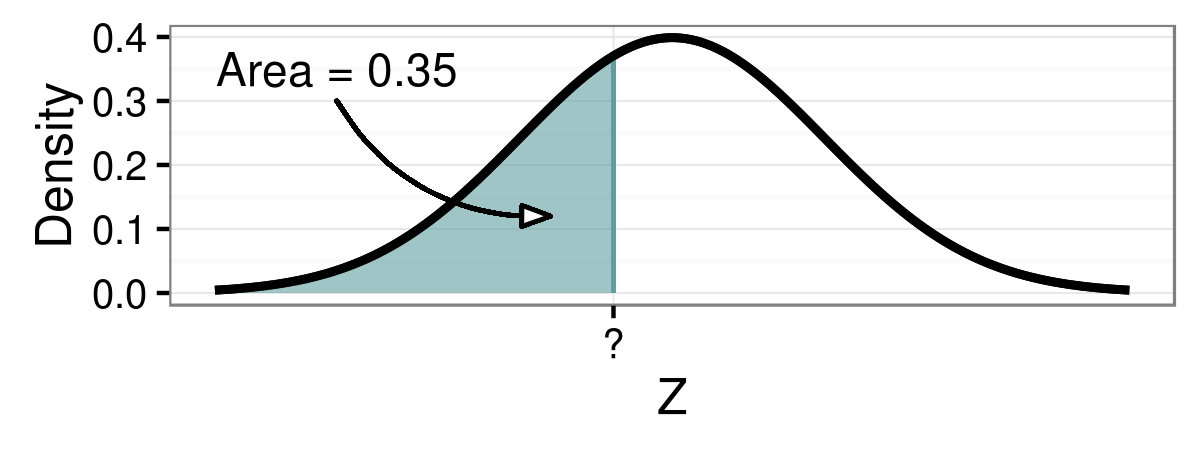
\includegraphics[width=4in]{../images/ch6_ex04}
\par}

\begin{itemize}
\pause\item $P(Z < \bv{-0.385}) = 0.35$
\end{itemize}
\end{exampleblock}
\end{frame}

\begin{frame}{Critical values}
\begin{block}{}
{\large In a standard normal distribution, the $z$-score separating usual outcomes from unusual outcomes is known as a \bt{critical value}.}
\begin{itemize}
\item The probability denoting unusual events is designated with $\alpha$ (alpha).
\item Then $z_\alpha$ is the critical value such that $P(Z > z_\alpha) = \alpha$
\end{itemize}
\end{block}

\medskip
{\centering
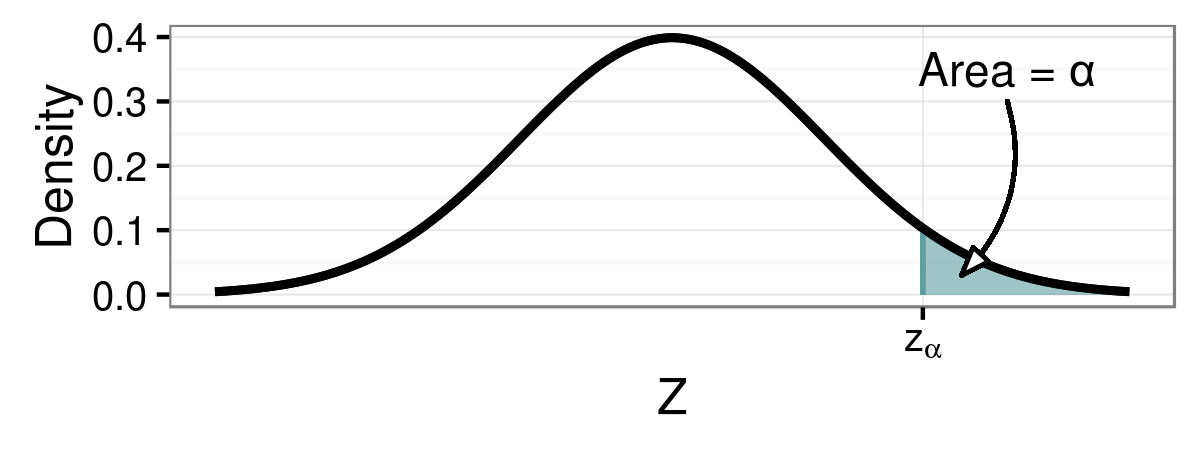
\includegraphics[width=4in]{../images/ch6_alpha}
\par}

\end{frame}

\begin{frame}{Critical values, example}
\begin{exampleblock}{Example}
Let $\alpha = 0.05$.\\
\medskip
Find the critical value for $\alpha$. That is, find $z_\alpha$ or $z_{0.05}$.
\begin{itemize}
\pause\item $z_\alpha = 1.645$
\item $P(Z > z_\alpha) = \alpha$ or $P(Z < -z_\alpha) = \alpha$
\end{itemize}
\end{exampleblock}
\smallskip
{\centering
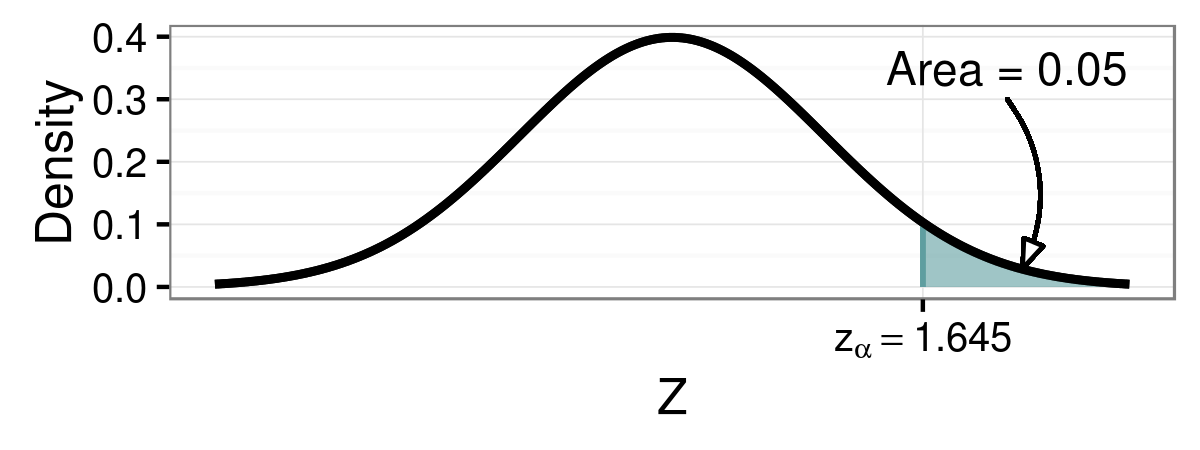
\includegraphics[width=4in]{../images/ch6_crit1}
\par}

\end{frame}


\begin{frame}{Critical values, example}
\begin{exampleblock}{Example}
Let $\alpha = 0.05$.\\
\medskip
Find the critical value for $\alpha/2$. That is, find $z_{\alpha/2}$ or $z_{0.025}$.
\begin{itemize}
\pause\item $z_{\alpha/2} = 1.96$
\item $P(Z < -z_{\alpha/2}) + P(Z > z_{\alpha/2}) = \alpha$
\end{itemize}
\end{exampleblock}
\smallskip
{\centering
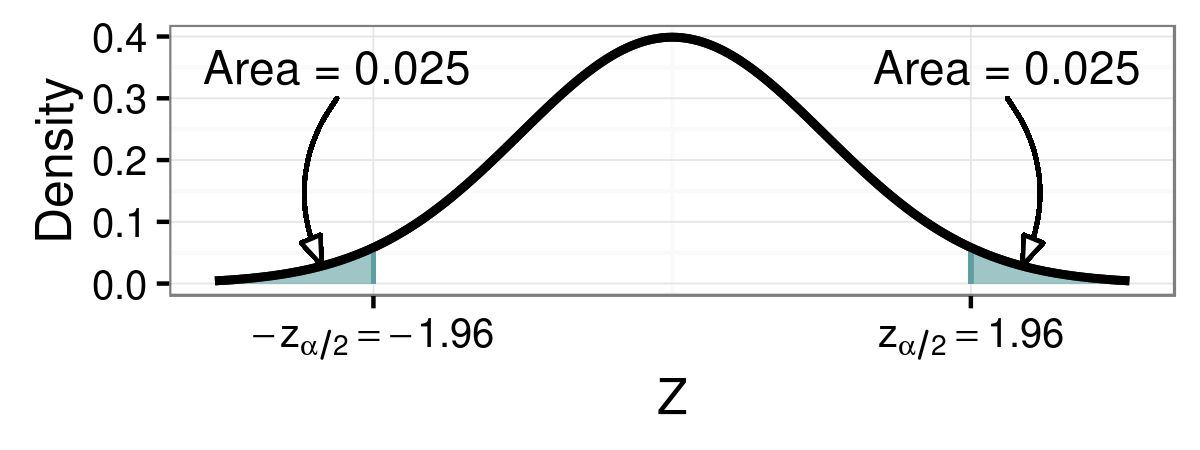
\includegraphics[width=4in]{../images/ch6_crit2}
\par}

\end{frame}

\begin{frame}<handout:0>{Group work}
\begin{block}{}
\large
\begin{itemize}
\item Complete question 1.
\end{itemize}
\end{block}
\end{frame}

% Section 6.2
\subsection{Real Applications of  Normal Distribution}

\begin{frame}{Non-standard normal distributions}
\begin{block}{}
Any value from a normal distribution, given the mean $\mu$ and standard deviation $\sigma$, can be converted into a standard normal $z$-score with the transformation,\\
\smallskip
{\centering
$\ds z = \frac {x - \mu}{\sigma}$
\par}
\smallskip
\begin{itemize}
\pause\item When using tables, this is the only way to find probabilities for non-standard normal random variables.
\pause\item With technology, this is no longer necessary.
\pause\item However, it is still useful to use $z$-scores for comparing values from different distributions.
\end{itemize}
\end{block}
\end{frame}

\begin{frame}{Z-score comparison, example}
\begin{exampleblock}{Example}
In the United States, adult women have a mean height of 63.7 in with a standard deviation of 5.96 in. Adult men have a mean height of 69.2 in with a standard deviation of 5.79 in.\\
\medskip
Jane is 71 inches tall and Rafael is 74 inches tall. Who is taller, relative to their genders? Are either of them unusually tall?
\begin{itemize}
\pause\item Jane: $\ds z = \frac {x - \mu}{\sigma} = \frac {71 - 63.7}{5.96} = 1.22$
\pause\item Rafael: $\ds z = \frac {74 - 69.2}{5.79} = 0.83$
\pause\item Jane is taller for a woman, than Rafael is for a man.
\pause\item Neither $z$-score is greater than 2 (or 1.96). Neither is unusual.
\end{itemize}
\end{exampleblock}
\end{frame}

\begin{frame}{Values in non-standard normal distributions}
\begin{block}{}
Similarly, $z$-scores can be converted into values in any other normal distribution with the following transformation,\\
\smallskip
{\centering
$\ds x = \mu + z \sigma$
\par}
\medskip
\end{block}

\pause
\begin{exampleblock}{Example}
A cruel statistics professor (not me) fails any student whose score on the final is less than 1.5 standard deviations below the mean. For one class, the scores on the final had a mean of 84.3 with a standard deviation of 7.8. What portion of the class does he fail? What is the boundary for failing scores for this class?
\begin{itemize}
\pause\item $P(Z < -1.5) = 0.067$
\pause\item $x = \mu + z \sigma = 84.3 + (-1.5) (7.8) = 72.6$
\end{itemize} 
\end{exampleblock}
\end{frame}

\begin{frame}{Probabilities, percentiles and critical values}
\begin{block}{}
Probabilities, percentiles and critical values can all be found for non-standard normal distributions.
\begin{itemize}
\item Using tables, values are converted to z-scores, the relevant table look-up performed, and then converted back into original distribution.
\item Again, technology makes the process easier.
\end{itemize}
\end{block}
\end{frame}


\begin{frame}{Non-standard normal distributions, example}
\begin{exampleblock}{Example}
An amusement park has made safety their highest priority. They design all their rides to have zero chance of causing serious head trauma, as long as the rider is under 78 inches tall. What proportion of men are in danger at this park?
\begin{itemize}
\pause\item $X_m \sim N(69.2, 5.79)$
\pause\item $P(X_m > 78) = \bv ?$
\pause\item $P(X_m > 78) = \bv{0.064}$
\end{itemize}

\end{exampleblock}
\end{frame}

\begin{frame}{Non-standard normal distributions, example}
\begin{exampleblock}{Example}
The amusement park is designing a new ride. It wants make sure that 85\% of adult women can ride it safely. What is the maximum height the ride should be designed for?
\begin{itemize} 
\pause\item $X_f \sim N(63.7, 5.96)$
\pause\item $P(X_f <  \bv ?) = 0.85$
\pause\item $P(X_f <  \bv{69.88}) = 0.85$
\end{itemize}
\end{exampleblock}
\end{frame}

\begin{frame}{Non-standard normal distributions, example}
\begin{exampleblock}{Example}
The amusement park is growing weary of accommodating the very tall and the very short. It has decided to exclude the most extreme heights among adult men. But it doesn't want to lose to much business, so it will only exclude 5\% of the adult male population. What are the critical values for the tallest and shortest men, for a total of 5\%?
\begin{itemize} 
\pause\item $X_m \sim N(69.2, 5.79), \qquad \alpha = 0.05$
\pause\item $z_{\alpha/2} = z_{0.025} = 1.96$
\pause\item $P(X_m <  \bv{57.85}) = 0.025, \qquad P(X_m >  \bv{80.55}) = 0.025$
\end{itemize}

\end{exampleblock}
\end{frame}

\begin{frame}<handout:0>{Group work}
\begin{block}{}
\large
\begin{itemize}
\item For questions 2 and 3, complete part (a).
\end{itemize}
\end{block}
\end{frame}

% Section 6.3
\subsection{Sampling Distributions and Estimators}

\begin{frame}{Samples, statistics and sampling distributions}
\begin{block}{}
\large Recall, a \bt{sample} is a subset of a population. A \bt{statistic} is a value calculated from the data of a sample.\\
\medskip
A \bt{sampling distribution} is a probability distribution of a statistic from all possible samples of a certain size from a population.
\end{block}

\pause
\begin{block}{}
\large
A sampling distribution is a mathematical construction. Understanding how statistics from samples are distributed, allows judgements to be made about the predictive value of individual samples that might be collected in real life.
\end{block}
\end{frame}

\begin{frame}{Sampling distributions, example}
\begin{exampleblock}{Example}
\large
Suppose we have a population of 3 values: \{ 1, 2, 3 \}.  \\
\pause\medskip
There are 9 possible samples (with replacement) of size 2:\\
\{ (1,1), (1,2), (1,3), (2,1), (2,2), (2,3), (3,1), (3,2), (3,3) \}\\
\pause\medskip
The sample means, $\bar x$, are:
\{ 1, 1.5, 2, 1.5, 2, 2.5, 2, 2.5, 3 \}\\
\pause\medskip
The sampling distribution of the sample means is:\\
\smallskip
{\centering
\begin{tabular}{c | c  c  c  c  c}
$\bar x$ & 1 & 1.5 & 2 & 2.5 & 3\\
\hline
Prob & 1/9 & 2/9 & 3/9 & 2/9 & 1/9
\end{tabular}
\par}
\end{exampleblock}.
\\
{\centering
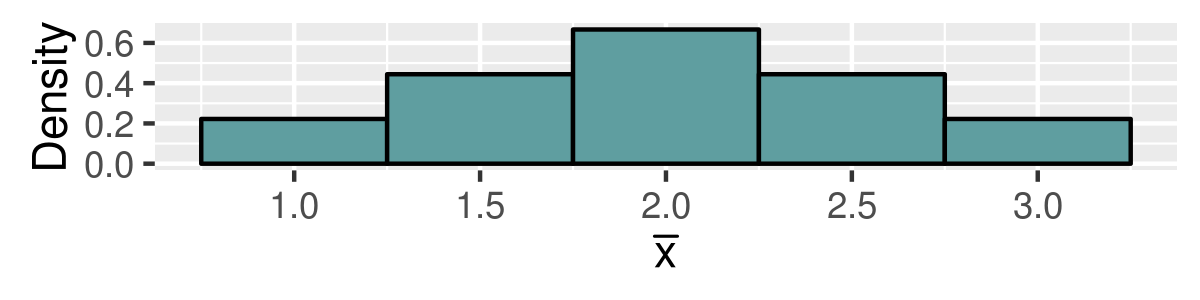
\includegraphics[width=4in]{../images/ch6_samp_dist}
\par}

\end{frame}

\begin{frame}{Estimators}
\begin{block}{}
\large An \bt{estimator} is statistic from a sample used to estimate a population parameter. 
\begin{itemize}
\pause\item For example, the sample mean $\bar x$ can be used to estimate the population mean $\mu$.
\pause\item Any statistic can be used as an estimator. The population mean could be estimated by the constant value 4, but this is almost always a poor estimate (unless the population mean is, in fact, 4).
\end{itemize}
\end{block}
\end{frame}

\begin{frame}{Unbiased estimators}
\begin{block}{}
\large If the expected value of an estimator, as calculated from the sampling distribution, is equal to the parameter it is estimating, the estimator is said to be \bt{unbiased}. 
\begin{itemize}
\pause\item Sample mean, $\bar x$, is an unbiased estimator of population mean. $\mu$.
\pause\item Sample standard deviation, $s$, is an unbiased estimator of population standard deviation, $\sigma$.
\pause\item Sample proportion, $\hat p$, is an unbiased estimator for population proportion, $p$.
\begin{itemize}
\item It is common to use $\pi$ for population proportions, but we will stick to the books notation. 
\end{itemize}
\end{itemize}
\end{block}

\pause
\begin{alertblock}{}
Recall, sample standard deviation is calculated as 
\[s = \sqrt{\frac 1 {n-1} \sum (x - \bar x)^2}\]
\end{alertblock}
\end{frame}

% Section 6.4
\subsection{The Central Limit Theorem}

\begin{frame}{Central Limit Theorem}
\begin{block}{}
\large
The \bt{Central Limit Theorem} (CLT) says that, given
\begin{itemize}
\pause\item $X$ is a random variable for a population with a mean $\mu$ and standard deviation $\sigma$
\pause\item Sampling distribution $S_{\bar x}$ of sample means $\bar x$ for samples of size $n$
\end{itemize}
\pause Then,
\begin{itemize}
\item As $n$ increases, $S_{\bar x}$ approaches a normal distribution
\pause\item The mean of $S_{\bar x}$, denoted $\mu_{\bar x}$, is $\mu$
\pause\item The standard deviation of $S_{\bar x}$, denoted $\sigma_{\bar x}$ and known as the \bt{standard error}, is $\ds \frac \sigma {\sqrt n}$  
\end{itemize}
\end{block}
\end{frame}

\begin{frame}{Central Limit Theorem demonstration}
\begin{block}{}
\large
For a demonstration of the Central Limit Theorem in action:
\begin{itemize}
\item \url{https://seighin.shinyapps.io/clt_demo/}
\end{itemize}
\end{block}
\end{frame}

\begin{frame}{Central Limit Theorem, example}
\begin{exampleblock}{Example}
\large
In the United States, adult women have a mean height of 63.7 in with a standard deviation of 5.96 in. \\
\medskip
What is the probability that a sample of 10 adult women will have a mean height of less than 69.88 inches,
\begin{itemize}
\pause\item The mean of the sample means is 63.7
\pause\item The standard deviation of the sample means, or standard error, is $\ds \frac {5.96}{\sqrt{10}} = 1.88$  
\pause\item $P(S_{\bar x} < 69.88) = 0.9995$
\end{itemize}
\end{exampleblock}

\end{frame}

\begin{frame}{Thoughts on CLT}
\begin{block}{}
\large
\begin{itemize}
\item If the population $X$ has a normal distribution, the sampling distribution $S_{\bar x}$ will have a normal distribution regardless of sample size $n$.
\pause\item If $X$ is not normally distributed, how normal $S_{\bar x}$ is, or how quickly it becomes normal as $n$ increases, depends on how not normal $X$ is.
\pause\item The rule of thumb generally used is, if sample size is $n=30$ or greater, $S_{\bar x}$ can be considered normal.
\end{itemize}

\end{block}

\pause
\begin{alertblock}{Remember\ldots}
The Central Limit Theorem applies to the distribution of estimators from samples, not the distribution of individual samples.
\end{alertblock}
\end{frame}

\begin{frame}{Elevator example}
\begin{exampleblock}{Example}
Suppose an elevator has a maximum capacity of 16 passengers with a total weight of 2500 lb. Assume male weights follow a normal distribution with a mean of 182.9 lb and a standard deviation of 40.8 lb. \\
\medskip
Find the probability that 1 randomly selected male has a weight greater than 156.25 lb (2500 lbs./16).
\begin{itemize}
\pause\item $X \sim N(182.9, 40.8)$
\pause\item $P( X > 156.25) = 0.743$
\end{itemize}
\pause\medskip
Find the probability that a sample of 16 males have a mean weight greater than 156.25 lb. 
\begin{itemize}
\pause\item $\mu_{\bar x} = 182.9, \qquad \sigma_{\bar x} = \frac {40.8}{\sqrt{16}} = 10.2$
\pause\item $S_{\bar x} \sim N(182.9, 10.2)$
\pause\item $P(S_{\bar x} > 156.25) = 0.996$
\end{itemize}
\end{exampleblock}
\end{frame}

\begin{frame}<handout:0>{Group work}
\begin{block}{}
\large
\begin{itemize}
\item For questions 2 and 3, complete part (b).
\end{itemize}
\end{block}
\end{frame}

\end{document}